%notfulltexdoc
\section{Theory}
\subsection{Bluetooth Low Energy}

Bluetooth low energy (or BLE for short) is a wireless personal area network technology aimed at applications in health care, fitness, security, and home entertainment. 
It allows peripheral devices such as smart phones, medical (heart rate, pressure) sensors and wireless earphones to transmit data within a personal area network. 
Compared to the classic Bluetooth, its purpose is to provide reduced power consumption while maintaining a similar range of communication. 
It saves power by sending small bursts of data as opposed to a continuous stream as used in classic Bluetooth technologies. 
This section of the report details the theory behind BLE and its use cases relevant to the project \cite{gatt}.\\

The purpose of BLE in this project is for it to allow the pair of Nucleo and Discovery boards to communicate data over BLE to a smart phone which then transmits that data to the internet. 
BLE works similarly to Bluetooth, in which a \textit{Central Device} scans for \textit{Peripheral Devices} which \textit{advertise} their personal area networks. 
At this point, once the central and peripheral device connect to one another, one acts as the \textit{Client Device} which receives data from the \textit{Server Device}.\\

For sending data, the server does so by packaging its data within a \textit{Value} under a \textit{Characterstic}, each of which are packaged within a \textit{Service}, this hierarchy of data is part of the \textit{GATT Profile Hierarchy}.\\
One can see this hierarchy within the following \hyperref[fig:uiscreenshot]{Figure \ref{fig:gatt}} \cite{gatt}.\\
\begin{figure}[h]
	\caption{GATT Profile Hierarchy}\label{fig:gatt}
	\begin{center}
		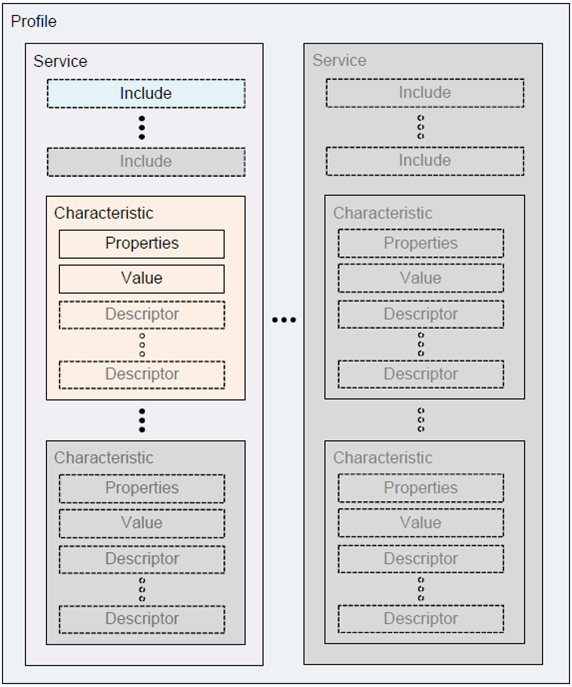
\includegraphics[width=3 inch]{GATT_Profile_Hierarchy.png}
	\end{center}
\end{figure}

Each server device has only one GATT profile, but within the profile, it may have multiple services, which represent different features. 
For example, one service can be for a heart rate sensor, and another for a pressure sensor. 
In this project, there is only one custom made service. 
A service may have multiple characteristics, which represents different data. 
For example, one characteristic can for a heart rate measurement and one can be for configuration settings for the heart rate sensor.
Within each characteristic, there is a \textit{Value}, the actual data. 
Then there contains one or many \textit{Descriptors}, which describe a value. 
Finally, \textit{Properties} contain the read, write and notify permissions for that characteristic values.\\